\documentclass[12pt]{article}
%\usepackage{tkiz}

\usepackage[utf8]{inputenc}
\usepackage[french]{babel}
\usepackage{amsmath,amsthm,amsfonts,amssymb}
\usepackage{lmodern}
\usepackage[top=2.4cm,bottom=2.4cm,left=2cm,right=2cm]{geometry}
\usepackage{hyperref}
\usepackage{multicol}
\usepackage{enumitem}
\usepackage{listings}
\usepackage[dvipsnames]{xcolor}
\usepackage{tikz}

%\date{}
\title{{\bf  Génie logiciel} \\
	Notes du cours de 18/11  \\
	{\small L3 Informatique appliquée 2022-2023} \\
	{\it \small MABROUK Fayez}}
\begin{document}
	\maketitle
	\newpage
	\section{Diagramme de séquence}
	\subsection{Prise en compte du temps}
		\begin{figure}[!hbtp]
		\centering
		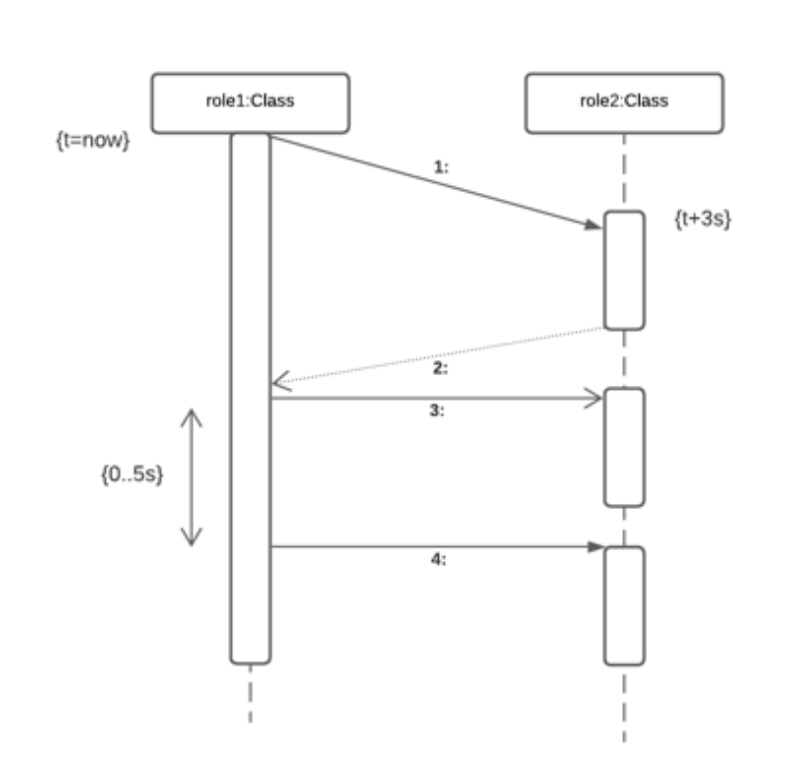
\includegraphics[scale=0.75]{Capture1.PNG}
		%\caption{Légende de l'image}
	\end{figure}
	\begin{itemize}
		\item[* ] Si nécessaire, vous pouvez donner une indication de temps
		dans votre diagramme de séquence.
		diagramme.
		\item[* ] Entre parenthèses.
	\end{itemize}
\subsection{Création et destruction d'objets}
	\begin{figure}[!hbtp]
	\centering
	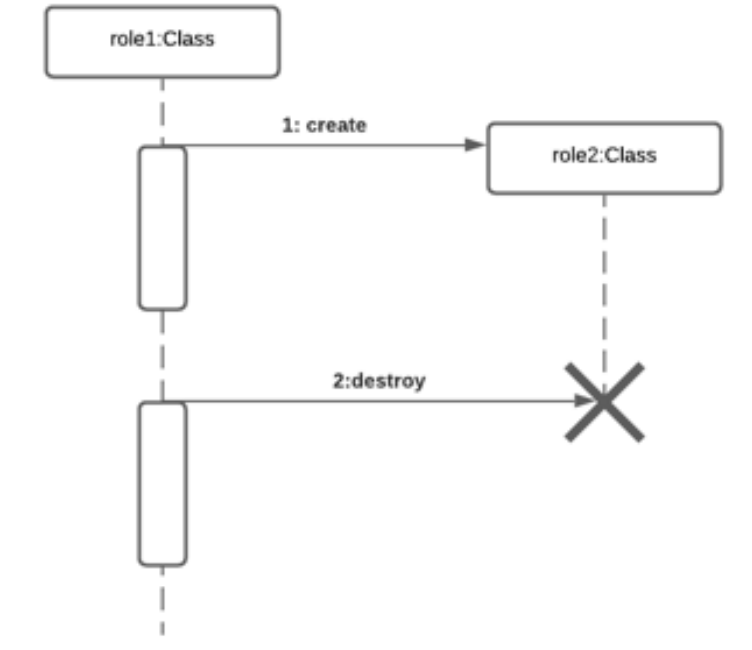
\includegraphics[scale=0.75]{Capture2.PNG}
	%\caption{Légende de l'image}
\end{figure}
\begin{itemize}
	\item[* ] Possibilité de créer et de détruire
	objets.
	\item[* ]  Pour créer : démarrer la ligne de vie au niveau du
	message.
	\item[* ] Pour détruire : mettre une croix.
\end{itemize}
\subsection{Un exemple simple}
	\begin{figure}[!hbtp]
	\centering
	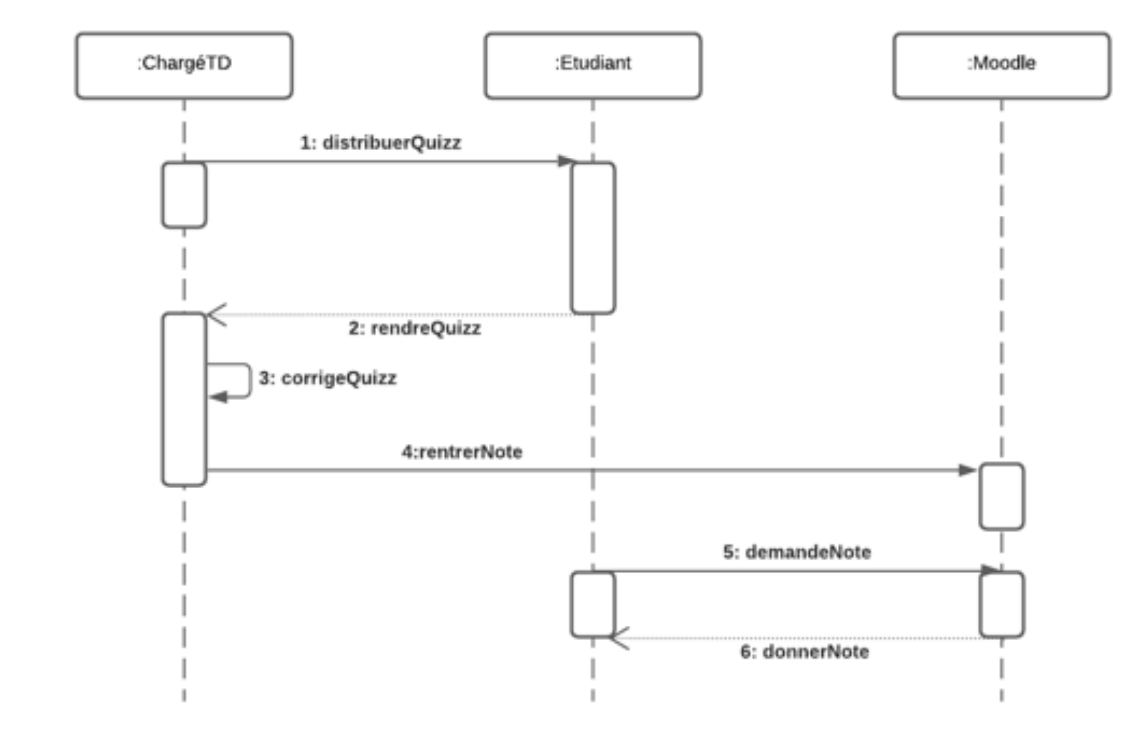
\includegraphics[scale=0.75]{Capture3.PNG}
	%\caption{Légende de l'image}
\end{figure}
\subsection{Diagrammes de séquence organisés - référence}
\begin{itemize}
	\item[* ] Comme nous l'avons vu dans l'exemple précédent, les diagrammes de séquence peuvent devenir
	encombrés.
	\item[* ] Vous pouvez utiliser des "fragments de référence" pour organiser logiquement vos diagrammes de séquence.
	\item[* ] Pour définir le diagramme de séquence à utiliser comme référence : encadrez avec "sd : nom
	du diagramme de séquence".
	\item[* ] sd = diagramme de séquence.
\end{itemize}
\subsection{Diagrammes de séquence organisés - alternatives}
\begin{itemize}
	\item[* ] Possibilité de définir des alternatives, sous la forme de "if then else".
	\item[* ] Note : possibilité d'avoir des "else ifs" (par l'ajout de lignes en pointillés).
\end{itemize}
\newpage
	\begin{figure}[!hbtp]
	\centering
	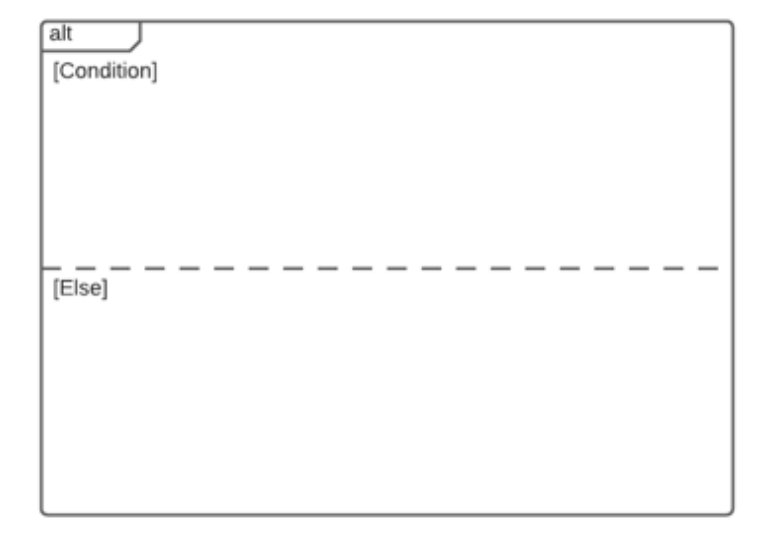
\includegraphics[scale=0.75]{Capture4.PNG}
	%\caption{Légende de l'image}
\end{figure}
\subsection{Diagrammes de séquence organisés - option}
\begin{itemize}
	\item[* ] Possibilité de définir une option, sous la forme de "if then".
	\begin{figure}[!hbtp]
		\centering
		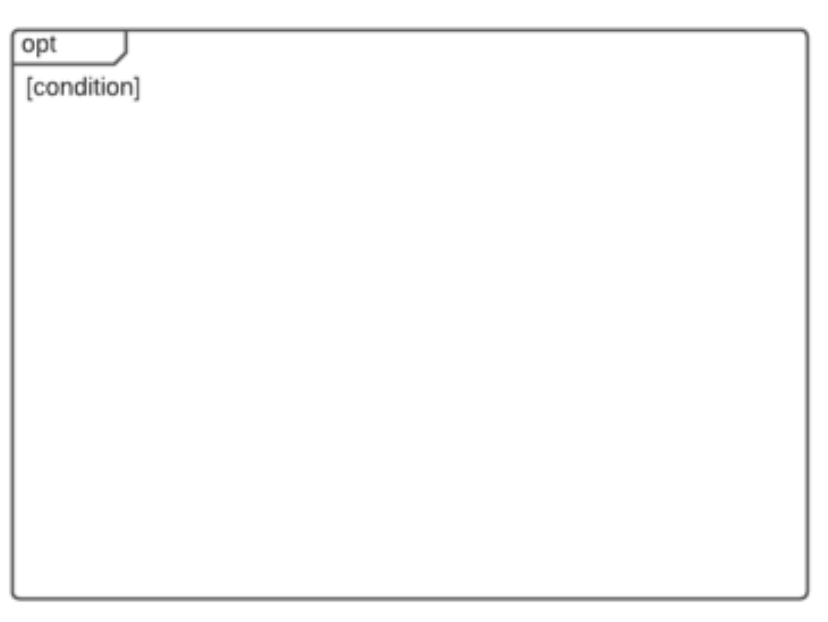
\includegraphics[scale=0.75]{Capture5.PNG}
		%\caption{Légende de l'image}
	\end{figure}
\end{itemize}
\subsection{Diagrammes de séquence organisés - boucles}
\begin{itemize}
	\item[*] Possibilité d'utiliser des boucles, entre deux nombres (min et max) et/ou jusqu'à ce que
	la condition soit vraie.
\end{itemize}
\newpage
\begin{figure}[!hbtp]
	\centering
	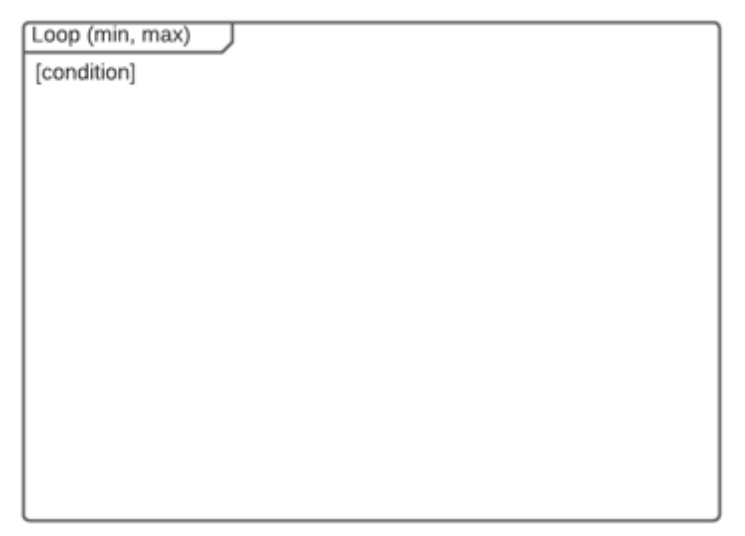
\includegraphics[scale=0.75]{Capture6.PNG}
	%\caption{Légende de l'image}
\end{figure}
\subsection{Diagrammes de séquence organisés - pause(break)}
\begin{itemize}
	\item[*] Quand la condition est vraie :
	\begin{itemize}
		\item[*] Exécute l'instruction à l'intérieur du module de rupture.
		\item[* ] quitte le fragment contenant le module de rupture.
		
	\end{itemize}
\end{itemize}
\begin{figure}[!hbtp]
	\centering
	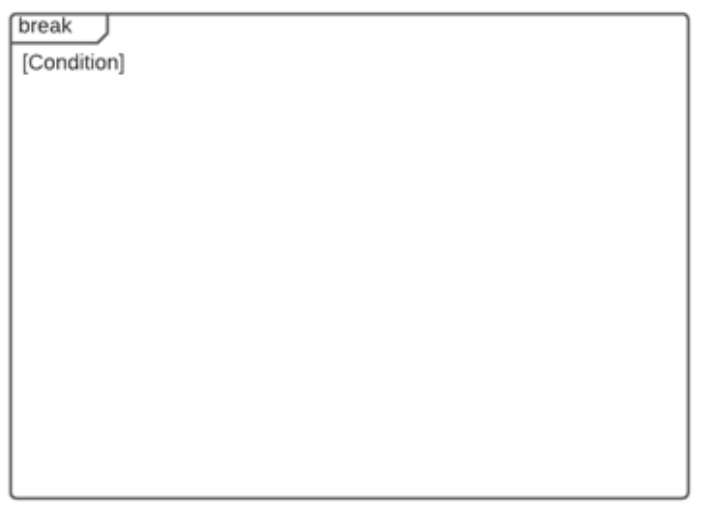
\includegraphics[scale=0.75]{Capture7.PNG}
	%\caption{Légende de l'image}
\end{figure}
\subsection{Diagrammes de séquence organisés - Négation}
\begin{itemize}
	\item[*] Définit une séquence qui est strictement interdite.
\end{itemize}
\newpage
\begin{figure}[!hbtp]
	\centering
	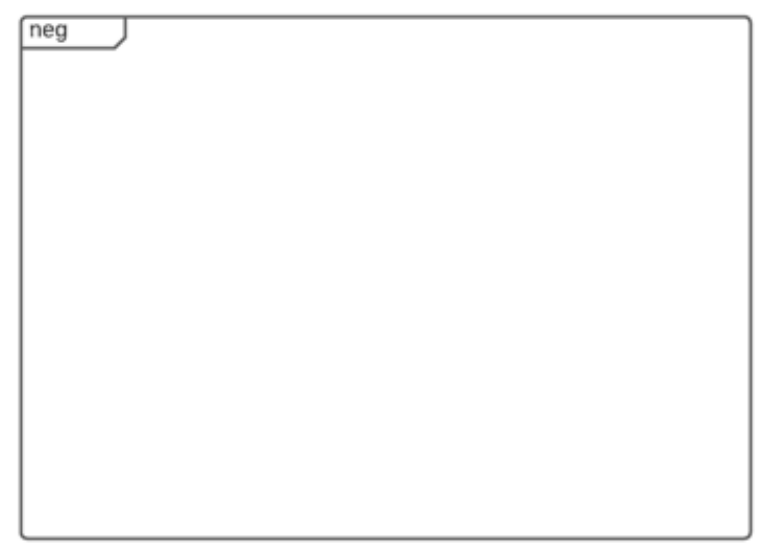
\includegraphics[scale=0.75]{Capture8.PNG}
	%\caption{Légende de l'image}
\end{figure}
\subsection{Diagrammes de séquence organisés - Parallélisme}
\begin{itemize}
	\item[*] Définit deux fragments qui sont exécutés simultanément.
\end{itemize}
\begin{figure}[!hbtp]
	\centering
	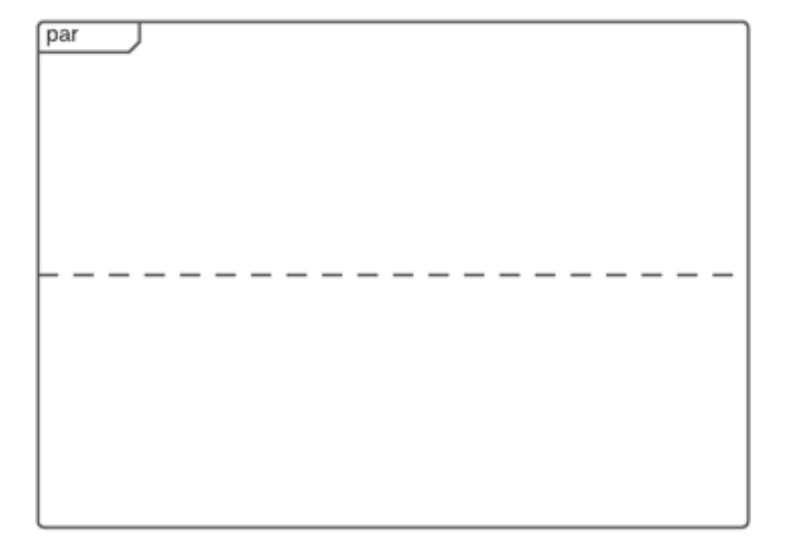
\includegraphics[scale=0.75]{Capture9.PNG}
	%\caption{Légende de l'image}
\end{figure}
\subsection{Diagrammes de séquence organisés - Critique}
\begin{itemize}
	\item[*] Définit un fragment qui ne peut pas être interrompu.
\end{itemize}
\newpage
\begin{figure}[!hbtp]
	\centering
	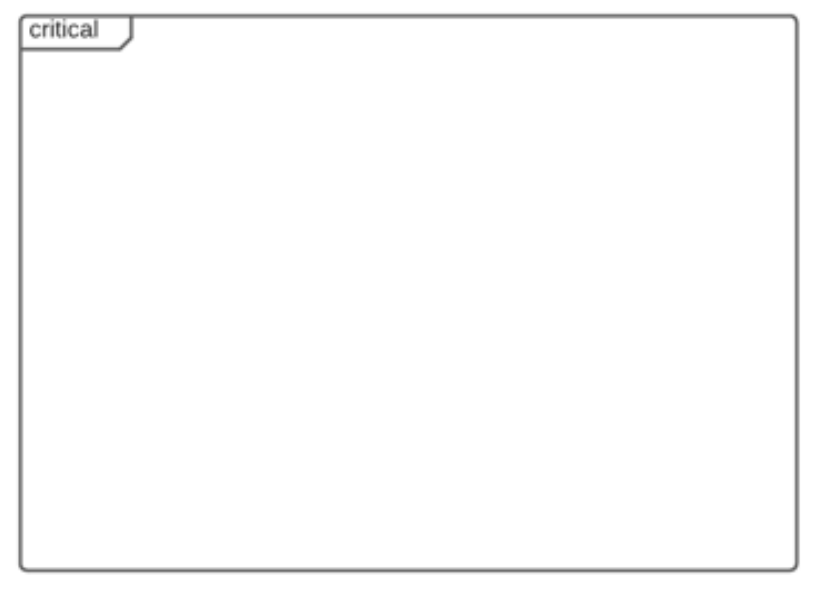
\includegraphics[scale=0.75]{Capture10.PNG}
	%\caption{Légende de l'image}
\end{figure}
\subsection{Conclusion}

\begin{itemize}
	\item[*] Les diagrammes de séquence sont utiles pour :
	\begin{itemize}
		\item[*] montrer comment les objets interagissent les uns avec les autres.
		\item[* ] il peut également être utile, en affinant les objets, de "découvrir" de nouveaux objets et leurs méthodes.
	\end{itemize}
	\item[* ] Ils peuvent devenir rapidement complexes.
	\item[* ] Ils doivent faire référence à un cas d'utilisation.
\end{itemize}
\newpage
\begin{figure}[!hbtp]
	\centering
	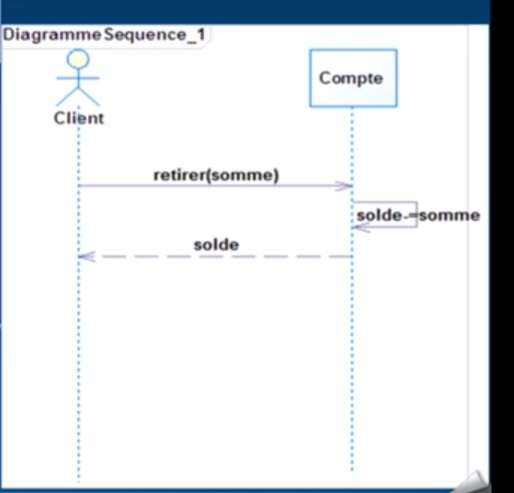
\includegraphics[scale=0.5]{Capture11.jpg}
	%\caption{Légende de l'image}
\end{figure}
\begin{figure}[!hbtp]
	\centering
	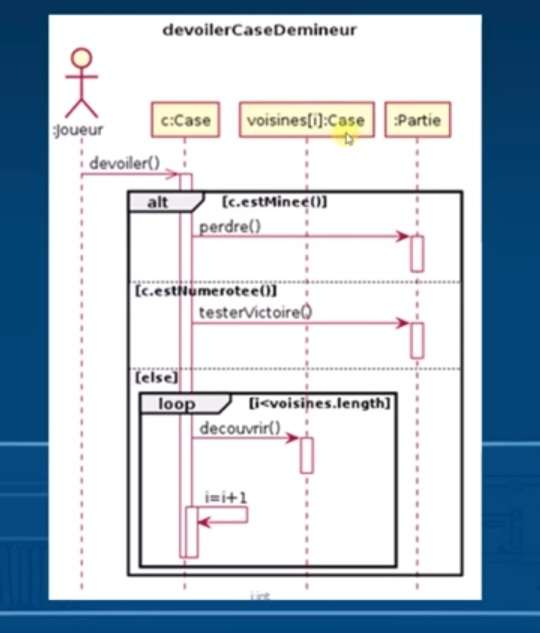
\includegraphics[scale=0.5]{Capture12.jpg}
	%\caption{Légende de l'image}
\end{figure}
\end{document}